\documentclass[a4paper,12px]{article}
\usepackage{graphicx}
\usepackage[english]{babel}
\usepackage{fullpage}
\usepackage{xfrac}
\usepackage{fancyhdr}
\usepackage{lastpage}
\usepackage{xifthen}
\usepackage[linesnumberedhidden, titlenotnumbered]{algorithm2e}
\usepackage{lipsum}
\usepackage{hyperref}
\usepackage{array}
\usepackage{tabularx}
\usepackage{caption}
\usepackage{amsfonts}
\usepackage{amssymb}
\usepackage{amsmath}
\usepackage{mathtools}
\usepackage{placeins}
\usepackage{enumitem}
\usepackage[noabbrev]{cleveref}
\usepackage[utf8]{inputenc}
\usepackage{multirow}

\usepackage{minted}
\usepackage{listings}
\usepackage{dsfont}
\usepackage{units}
\usepackage{epstopdf}

\pagestyle{fancy}
\lhead{\includegraphics[width=7cm]{logoUvA}}
\rhead{\footnotesize \textsc {Report\\ \opdracht}}
\lfoot%
{%
    \footnotesize \studentA%
    \ifthenelse{\isundefined{\studentB}}{}{\\ \studentB}
    \ifthenelse{\isundefined{\studentC}}{}{\\ \studentC}
    \ifthenelse{\isundefined{\studentD}}{}{\\ \studentD}
    \ifthenelse{\isundefined{\studentE}}{}{\\ \studentE}
}
\cfoot{}
\rfoot{\small \textsc {Page \thepage\ of~\pageref{LastPage}}}
\renewcommand{\footrulewidth}{0.5pt}

\fancypagestyle{firststyle}
{%
    \fancyhf{}
    \renewcommand{\headrulewidth}{0pt}
    \chead{\includegraphics[width=7cm]{logoUvA}}
    \rfoot{\small \textsc {Page \thepage\ of~\pageref{LastPage}}}
}

\setlength{\topmargin}{-0.3in}
\setlength{\textheight}{630pt}
\setlength{\headsep}{40pt}
\setlength{\parindent}{0pt}

% =================================== DOC INFO ===================================

\newcommand{\opdracht}{Theoretical Excercises}
\newcommand{\titel}{Labs 4}
\newcommand{\docent}{Alban Ponse, Bob Diertens}
\newcommand{\cursus}{Theoretische aspecten van de Programmatuur}
\newcommand{\vakcode}{}
\newcommand{\datum}{\today}
\newcommand{\studentA}{Maico Timmerman}
\newcommand{\uvanetidA}{10542590}
%\newcommand{\studentB}{Tim van Zalingen}
\newcommand{\uvanetidB}{10784012}
% \newcommand{\studentC}{Boudewijn Braams}
\newcommand{\uvanetidC}{10401040}
% \newcommand{\studentD}{Govert Verkes}
\newcommand{\uvanetidD}{10211748}
%\newcommand{\studentE}{Naam student 5}
\newcommand{\uvanetidE}{UvAnetID student 5}

% ===================================  ===================================

\begin{document}
\thispagestyle{firststyle}
\begin{center}
    \textsc{\Large \opdracht}\\[0.2cm]
    \rule{\linewidth}{0.5pt} \\[0.4cm]
    {\huge \bfseries \titel}
    \rule{\linewidth}{0.5pt} \\[0.2cm]
    {\large \datum\\[0.4cm]}

    \begin{minipage}{0.4\textwidth}
        \begin{flushleft}

            \emph{Student:}\\
            {\studentA\\ {\small \uvanetidA\\[0.2cm]}}
            \ifthenelse{\isundefined{\studentB}}{}{\studentB\\ {\small \uvanetidB\\[0.2cm]}}
        \end{flushleft}
    \end{minipage}~%
    \begin{minipage}{0.4\textwidth}
        \begin{flushright}
            \emph{Lecturers:} \\
            \docent\\[0.2cm]
            \emph{Course:} \\
            \cursus\\[0.2cm]
            % \emph{Student:}\\
            \ifthenelse{\isundefined{\studentC}}{}{\studentC\\ {\small \uvanetidC\\[0.2cm]}}
            \ifthenelse{\isundefined{\studentD}}{}{\studentD\\ {\small \uvanetidD\\[0.2cm]}}
            \ifthenelse{\isundefined{\studentE}}{}{\studentE\\ {\small \uvanetidE\\ [0.2cm]}}
        \end{flushright}
    \end{minipage}\\[1 cm]
\end{center}


% =================================== CONTENTS ===================================

% \tableofcontents

\newcommand{\Sum}[2]{\sum^{#2}_{#1}}
\newcommand{\E}[1]{{\mathbb{E}\left[#1\right]}}
\newcommand{\var}[1]{{\text{var}\left[#1\right]}}
\newcommand{\diffpart}[1]{\frac{\partial}{\partial{} #1}}
\newcommand{\?}{\stackrel{?}{=}}
\newcommand{\intinf}{\int\limits_{-\infty}^{\infty}}
\newcommand{\intnulinf}{\int\limits_{0}^{\infty}}
\newcommand{\intpi}{\int\limits_{0}^{2\pi}}
\newcommand{\argmin}[1]{\underset{#1}{\mathop{\mathrm{argmin}}}}
\newcommand{\argmax}[1]{\underset{#1}{\mathop{\mathrm{argmax}}}}
\definecolor{bg}{rgb}{0.95,0.95,0.95}
% =================================== MAIN TEXT ===================================


\section*{Factory 1}
\subsection*{1. Factory construction}

Factory1 consists of 5 working cells, of which 2 have are concurrent cells. WC1
reads from the input and writes to either WC2 if it is an \verb|A| or to any of
the WC3 when the value is a \verb|B|. This is the only place guarded
expressions are needed, because products need to be splitted.

All other working cells can just communicate any product they receive to the
next cell using a simple sequence of instructions that can be seen below.

\begin{minted}{C++}
WCx = sum(p in PRODUCT,
          rec(IDx1, IDx2, p) .
          wcx(p) .
          snd(IDx2, IDx3, p)
       ) . WC2
\end{minted}

For any product, first receive that product from \verb|IDx1| and store it in
itself \verb|IDx2|. Then it it processed by the working cell: \verb|wcx(p)|,
after which is is send out again to the next receiver \verb|IDx3|.

All cells work the same way, with different channels. \verb|A| is processed by WC1, followed by WC2 and WC4.
\verb|B| is processed by WC1, followed by either WC31 or WC32 and finally WC4.

Factory1 can be seen in \autoref{fig:factory1}.

\begin{figure}[h]
    \centering
    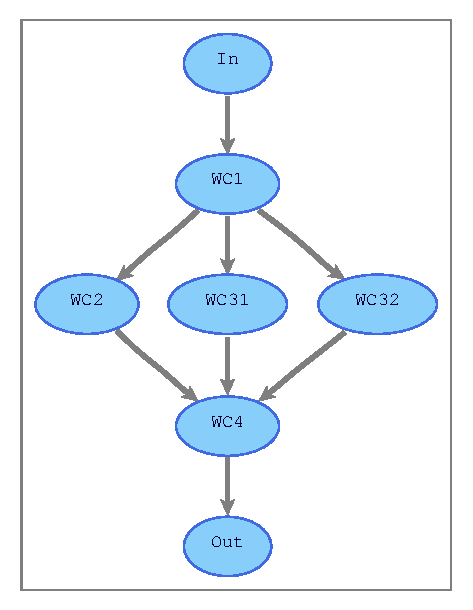
\includegraphics[width=0.4\linewidth]{Factory1/Factory1.eps}
    \caption{Factory1}
    \label{fig:factory1}
\end{figure}
\FloatBarrier%

\subsection*{2. Sequence conversion}

The sequence \verb|ABBA| can easily be converted by storing the first \verb|A|
in WC2 and then processing both \verb|B|. After both the \verb|B| have been
send to the output, the factory continues processing both \verb|A|. The trace for this can be seen
in the following listing.

\begin{minted}{C}
START Factory1
trace> atom input(A)            // input(A)
trace> comm comm(IN, ID1, A)
trace> atom wc1(A)
trace> atom input(B)            // input(B)
trace> comm comm(ID1, ID2, A)
trace> comm comm(IN, ID1, B)
trace> atom input(B)            // input(B)
trace> atom wc1(B)
trace> comm comm(ID1, ID31, B)
trace> atom wc31(B)
trace> comm comm(ID31, ID4, B)
trace> atom wc4(B)
trace> comm comm(ID4, OUT, B)
trace> atom output(B)           // output(B)
trace> comm comm(IN, ID1, B)
trace> atom input(A)            // input(A)
trace> atom wc1(B)
trace> comm comm(ID1, ID31, B)
trace> atom wc31(B)
trace> comm comm(ID31, ID4, B)
trace> atom wc4(B)
trace> comm comm(ID4, OUT, B)
trace> atom output(B)           // output(B)
trace> comm comm(IN, ID1, A)
trace> atom wc1(A)
trace> atom wc2(A)
trace> comm comm(ID2, ID4, A)
trace> comm comm(ID1, ID2, A)
trace> atom wc4(A)
trace> atom wc2(A)
trace> comm comm(ID4, OUT, A)
trace> atom output(A)           // output(A)
trace> comm comm(ID2, ID4, A)
trace> atom wc4(A)
trace> comm comm(ID4, OUT, A)
trace> atom output(A)           // output(A)
\end{minted}

\section{Factory2}

In Factory2 \verb|B| have to pass both WC3. Which means that whenever \verb|B|
is read from WC1, it first needs to be passed to the other WC3. i


In \autoref{fig:deadlock} can be seen that this factory can create a deadlock.
When both WC3 have read \verb|B| from WC1 and not yet pass it to other WC3, a
circular dependency arises.

To implement the handling of the ``halfproduct'', a combination of two sums had
to be created. While the following code would suffice, the arrows would not be
drawn correctly:

\begin{minted}{C}
WC31 = (
        (rec(ID1, ID31, B) .  wc31(B) .  snd(ID31, ID32, B1))
        + (rec(ID32, ID31, B) .  wc31(B2) .  snd(ID31, ID4, B))
        ) . WC31
\end{minted}

Instead the implementation for halfproduct has been implemented as following:
\begin{minted}{C}
WC31 = (sum(p in PRODUCT,
           rec(ID1, ID31, p) .
           wc31(p) .
           snd(ID31, ID32, B1))
    +  sum(p in PRODUCT,
           rec(ID32, ID31, p) .
           wc31(p) .
           snd(ID31, ID4, B))
    ) . WC31
\end{minted}

In \autoref{fig:deadlock} can be seen that this factory can create a deadlock.
When both WC3 have read \verb|B| from WC1 and not yet pass it to other WC3, a
circular dependency arises.

\begin{figure}[h]
    \centering
    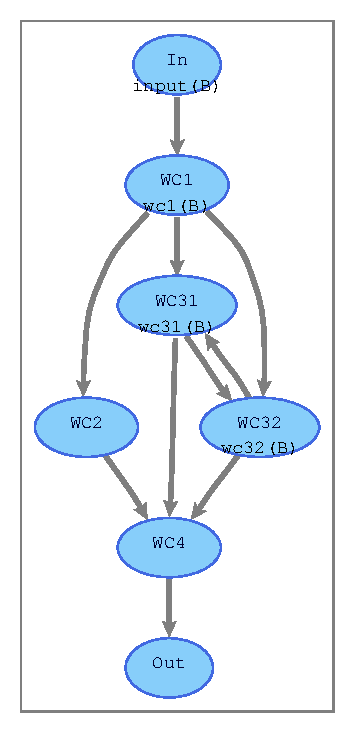
\includegraphics[width=0.4\linewidth]{Factory2/deadlock.eps}
    \caption{Factory with deadlock}
    \label{fig:deadlock}
\end{figure}
\FloatBarrier%

To solve this problem, a couple theoretical solutions can be though of. First
of, the traversing of B is changed to a sequential order. Thus \verb|B = WC31.
WC32|, this way, there are no options that deadlock is created. However it
makes the halfproduct \verb|B2| useless.

Another option is to use a parallel composition \verb=a||b= of the receive
action from WC1 and some form of locking communication to the other WC3. When a
WC3 receives an locking communication, it will only receive a halfproduct, and
not receive from WC1. This prevents that both work cells are stuck with a
halfproduct, which they can not pass.

% =================================== REFERENCES ===================================

% \clearpage

% \bibliographystyle{apalike}
% \bibliography{report}

\end{document}
